\documentclass[11pt]{article}

\usepackage[english]{babel}
\usepackage[a4paper,top=2.2cm,bottom=2.2cm,left=2.5cm,right=2.5cm]{geometry}
\usepackage{amsmath,amssymb}
\usepackage{algorithm}
\usepackage{algpseudocode}
\usepackage{booktabs}
\usepackage{float}
\usepackage{multirow}
\usepackage{graphicx}
\usepackage{caption}
\usepackage{microtype}
\usepackage[colorlinks=true,allcolors=blue]{hyperref}

\title{Understanding and decomposing group unfairness in collaborative filtering: the role of activity and rating eccentricity}
\title{Hidden Distributional Sources of Group Fairness\\
in Collaborative Filtering}
\author{Jorge Paz-Ruza \and Iris Domínguez-Catena \and Mikel Galar \and Amparo Alonso-Betanzos \and Bertha Guijarro-Berdiñas}
\date{}

\begin{document}
\maketitle

\begin{abstract}
Fairness evaluations of recommender systems commonly attribute differences in
error between user groups to group representation, sensitive attributes, or
stereotypical preferences. We argue that this view is incomplete for
collaborative filtering: the distribution of observed ratings also determines
what a model learns and which errors are visible at evaluation time. We
introduce an experimental framework for isolating hidden distributional
factors, like user activity, rating eccentricity and other psychosociological traits, and to discompose their effects on perceived group unfairness, both due to inductive model biases or disparate distributions. Across our experiments, measured group unfairness can be decomposed and understood by employing our proposed method, helping explain how and why collaborative filtering models favor one group over another. These
results challenge explanations of recommender group unfairness and motivate distribution-aware fairness analyses like our proposal.
\end{abstract}

\section{Introduction}
\label{sec:introduction}

Recommender systems learn from interactions that are neither uniformly
distributed nor independent of the users and items producing them. A user
with many observed interactions supplies a different training signal from a
user with only a few. Users and items also differ in how typical their
observed interactions are. These properties are usually treated as data
diagnostics, yet they can become ingredients of model disparity: they
influence the representations learned by a collaborative model and determine
which examples dominate an error metric.

This issue is particularly important for group fairness. Existing analyses
often organize fairness around protected-group representation, popularity, or
the possibility that a model reproduces social stereotypes
\cite{dwork2012,ekstrand2018,burke2017,mehrabi2021}. Those mechanisms matter,
but a recommender can show a group error gap even when the sensitive attribute
is not used by the model and even when group membership is assigned from artifical groups not representing real demographic factors.

The goal of this work is to provide a controlled way to characterize
distributional sources of group unfairness in Recommender systems. We consider not only known aspects of dyadic data like group representation and psycho-sociological criteria, but also hidden factors, namely user activity and rating eccentricity, which respectively describe how much concentrated the interaction population is, and how far an
observed rating departs from local user-item behavior. Eccentricity, in particular, is
motivated by a phenomenon recently described by Paz-Ruza et al.~\cite{pazruza2025},
who show that non-uniform observed-value distributions can make collaborative filtering models
 unassumingly favour ``average'' cases and perform disproportionately poorly on unexpected or ``eccentric'' interactions.

Our experimental question is not knowing what groups are more or less advantaged, but whether we can precisely attribute the perceived group unfairness of collaborative filtering models to a combination of known and hidden distributional factors disregarded in existing literature and practice. We make four main contributions, summarized on Figure \ref{fig:summary}:

\begin{figure}[H]
    \centering
    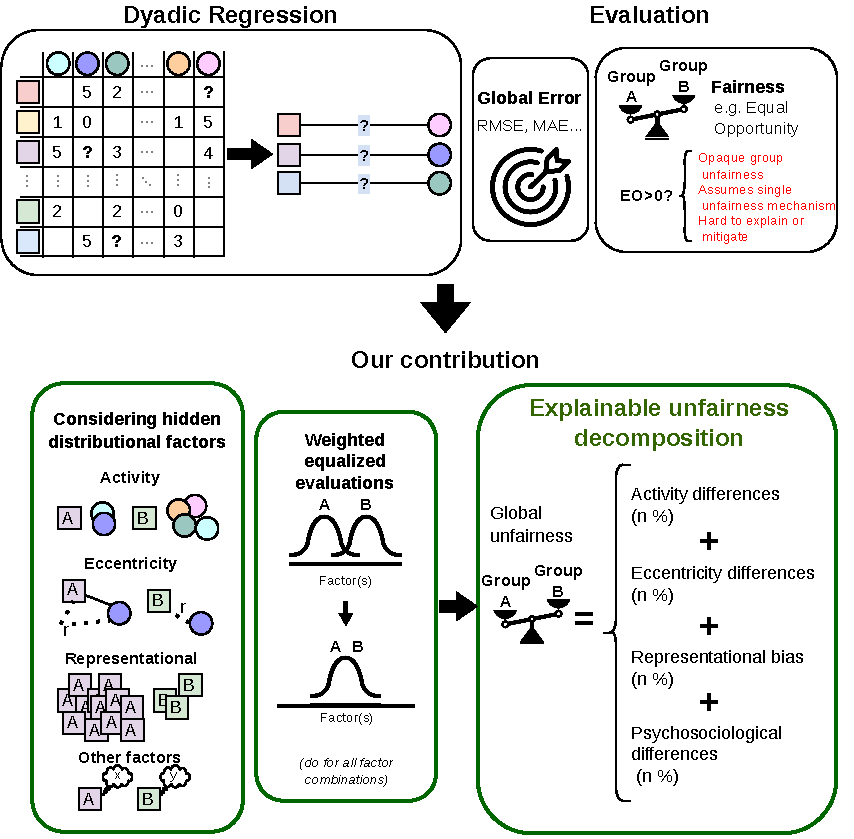
\includegraphics[width=.9\linewidth]{figures/DECOMPOSE_SUMMARY (1).pdf}
    \caption{Summary and rationale of this work's main contributions.}
    \label{fig:all-balancing-metrics}
\end{figure}


\begin{enumerate}
    \item We formulate activity and eccentricity as additional hidden distributional bias factors
    that can be analyzed independently of the demographic meaning of a group.
    \item We define a reproducible procedure for additive decomposition of the observed group unfairness of models into bias arising from eccentricity, activity, representational and other psychosociological factors that may be disparate between groups.
    \item We experiment in real-world collaborative filtering datasets considering natural, demographic group constructions as well as controlled, induced splits. Our results demonstrate the effectiveness of our method to decompose group unfairness sources.
    \item We prove the influence of activity and eccentricity disparities among groups in recommender fairness, challenging previous assumptions that only consider representational or psychosociological biases.
\end{enumerate}


\section{Background and Related Work}
\label{sec:related-work}

This section introduces the fairness perspective, collaborative-filtering
notation, and prior work that motivates our proposal for a decompositional algorithm of group unfairness treating activity and eccentricity as
possible distributional factors.

\subsection{Collaborative filtering task and notation}

Collaborative filtering predicts a user's preference for an item from a
sparse collection of observed user-item interactions. Let $\mathcal{U}$ and
$\mathcal{I}$ denote users and items, and let
$R\subseteq\mathcal{U}\times\mathcal{I}\times\mathbb{R}$ be the observed
interaction set. An element $(u,i,r_{ui})\in R$ records that user $u$ gave
item $i$ the rating $r_{ui}$. The user and item neighborhoods are
$R_u=\{(i,r_{ui}):(u,i,r_{ui})\in R\}$ and
$R_i=\{(u,r_{ui}):(u,i,r_{ui})\in R\}$. Their empirical means are
\begin{equation}
    \bar r_u=\frac{1}{|R_u|}\sum_{(i,r_{ui})\in R_u}r_{ui},
    \qquad
    \bar r_i=\frac{1}{|R_i|}\sum_{(u,r_{ui})\in R_i}r_{ui}.
\end{equation}

Models operating in collaborative filtering tasks are of the form $ r_{ui}=\phi(u,i,\cdots)$. Because the model $\phi$ learns from $R$, the composition of the observed
interactions affects both the evidence available for each representation and
the errors measured on later interactions.

\subsection{Fairness in recommender systems}

Fairness is not a single property in recommendation. It can concern users,
items, providers, exposure, utility, or the relation between predictions and
outcomes. Multisided formulations emphasize that different stakeholders can
have incompatible objectives \cite{burke2017}, while ranking work studies
exposure and attention rather than only prediction error
\cite{singh2018,biega2018}. Surveys have consequently distinguished
individual, group, consumer, provider, and multistakeholder notions of
fairness \cite{ekstrand2018,mehrabi2021}; in this work, we work on the popular subproblem of group fairness in direct ranking prediction tasks. 

Representation is often considered a central source of algorithmic disparity in Machine Learning. In Recommender systems, minority groups may have
fewer observations, less coverage, or systematically different interaction
patterns. In movie recommender systems, Gonzalez et al.~\cite{gonzalez2022} analyze bias and
unfairness in collaborative filtering and attributed representational bias to be the culprit of observed disparities.

These accounts, however they do not imply that representation is the only mechanism. In matrix factorization, observation
counts affect the amount of evidence available for user and item embeddings.
The values of those observations also affect the loss landscape, both in optimization and in evaluation. A group can
therefore be disadvantaged by the kinds of ratings it contributes, not only by
the number of users or ratings it contributes or a psychosociological difference in their behaviour. 

Further than evaluation, interventions to mitigate group unfairness include a myriad of pre-processing, in-processing,
and post-processing approaches, as well as constraints on ranking exposure or
group representation \cite{kamishima2012,hardt2016,celis2019}. These lines of
work establish important group-level and stakeholder-level and ethical positions to systematically reduce the overall group unfairness of collaborative filtering models, but they
do not by themselves explain what is the actual source of such biases, and do not investigate whether the internal distribution of collaborative
filtering evidence creates unequal prediction errors.

\subsection{Activity, popularity, and eccentricity}

Here, we describe different distributional factors that may affect group fairness in collaborative filtering: 
\begin{itemize}
    \item User activity and item popularity are the observation counts
\begin{equation}
    a_u=|R_u|,\qquad p_i=|R_i|.
    \label{eq:activity-popularity}
\end{equation}
Activity measures how much evidence is available for a user representation;
popularity measures how frequently an item appears in the observed
interaction graph. Item popularity bias has been extensively studied in learning-to-rank case, where items with large  $p_i$ in binary interaction graphs get disproportionately recommended at the expense of long-tail
items \cite{jannach2015,abdollahpouri2017,abdollahpouri2021}. In rating prediction tasks,
item popularity is part of the background mechanism that can shape learned item
representations, not affecting directly user group unfairness, while disparate user activity distributions may affect the quality of learning of the preferences for users of different groups, regardless of their overall group representation. 

\item For each observed interaction, define its local eccentricity by
\begin{equation}
    \epsilon_{ui}=\left|r_{ui}-\frac{\bar r_u+\bar r_i}{2}\right|.
    \label{eq:rating-eccentricity}
\end{equation}
The corresponding user-level eccentricity is the mean over that user's
observed interactions,
\begin{equation}
    e_u=\frac{1}{|R_u|}\sum_{(i,r_{ui})\in R_u}\epsilon_{ui}.
    \label{eq:user-eccentricity}
\end{equation}
Thus, $\epsilon_{ui}$ describes how atypical an
individual observation is relative to the expected for the dyad. 

Paz-Ruza et al.~\cite{pazruza2025} formalize eccentricity bias in dyadic
regression and introduce a metric to characterize overall model bias due to disproportionately punishing eccentric cases. Their analysis demonstrates
why global RMSE and MAE can hide structured errors, but do not translate it to individual or group fairness. In our work, eccentricity is not
itself a group definition; it is a candidate hidden factor that may help
explain why two groups receive different prediction errors.

\end{itemize}

\section{Proposal}
\label{sec:method}

This section defines the proposed diagnostic pipeline, consisting of evaluation- and training-time interventions on the measurement of group fairness biases in collaborative filtering. In particular, we propose to isolate and decompose how different individual distributional factors of the training and test data (e.g. user activity, rating eccentricity, group representation and other psychosociological factors) affect intrinsic model biases and group fairness metrics in the final evaluation. 


\subsection{Group constructions}
\label{sec:group-constructions}

Group membership is represented by a user-level label $g_u\in\{A,B\}$, so
every interaction by a user inherits that user's group. The proposal is
agnostic to how the two labels are obtained: they may denote observed groups,
controlled induced populations, or another user-level partition. The
precise group constructions and their parameters are implementation choices
reported in Section~\ref{sec:configuration}.

For a feature $x$ and population parameters $(\mu_A,\sigma_A)$ and
$(\mu_B,\sigma_B)$, the induced group probability is
\begin{equation}
 P(A\mid x)=\frac{\mathcal{N}(x;\mu_A,\sigma_A)}
 {\mathcal{N}(x;\mu_A,\sigma_A)+\mathcal{N}(x;\mu_B,\sigma_B)}.
\end{equation}
The label is sampled once per user. This construction deliberately separates a
distributional factor from a real-world protected attribute; the same formal
definition also covers any other user-level group assignment.

\subsection{Test-side weighting and EO decomposition}
\label{sec:test-intervention}

The test-side procedure attributes the model's overall observed group error
difference to hidden distributional factors. Holding the predictor and its
training data fixed, it constructs counterfactual evaluation distributions in
which activity and eccentricity are successively aligned between groups. The quantities needed for its decomposition are obtained through the weighted evaluations performed on four different conditions:
\begin{itemize}
    \item $\mathcal C_0$: no weighting;
    \item $\mathcal C_a$: activity weighting
    \item $\mathcal C_e$: eccentricity weighting
    \item $\mathcal C_{ae}$: joint activity--eccentricity weighting
\end{itemize}

Algorithm~\ref{alg:test-set-weighting} produces the evaluation quantities used
for attribution in six steps:
\begin{enumerate}
    \item It trains the checkpoint and restricts evaluation to test ratings
    whose users and items are represented in training
    (lines~\ref{alg:test-train}--\ref{alg:test-eligible}).
    \item It computes the training-set reference means and the pooled
    activity and eccentricity bins (lines~\ref{alg:test-means}--\ref{alg:test-bins}).
    \item It selects one of the four named conditions and, when required,
    assigns each eligible rating to its activity, eccentricity, or joint
    stratum.
    \item For each shared stratum, it counts the two groups, converts the
    counts to group proportions, and constructs the normalized common target
    (lines~\ref{alg:test-proportions}--\ref{alg:test-target}).
    \item It assigns importance weights, giving no weight to group-exclusive
    strata, and evaluates the unchanged checkpoint with those weights
    (lines~\ref{alg:test-weights}--\ref{alg:test-evaluate}).
    \item It records the condition-specific metrics for the EO decomposition
    (line~\ref{alg:test-aggregate}).
\end{enumerate}

\begin{algorithm}[H]
\caption{Test-set weighting and fixed-checkpoint evaluation}
\label{alg:test-set-weighting}
\begin{algorithmic}[1]
\Require Training set $T$, test set $V$; quantile counts $Q_a,Q_e$
\Ensure Predictions and metrics for conditions
       $\mathcal{C}=\{\mathcal C_0,\mathcal C_a,\mathcal C_e,\mathcal C_{ae}\}$
\State Train one model $M$ on $T$ and save its checkpoint
    \label{alg:test-train}
\State $E\gets\{v\in V:u(v)\in U(T)\ \land\ i(v)\in I(T)\}$
    \label{alg:test-eligible}
\State Compute $\bar r_u$ and $\bar r_i$ using $T$ only
    \label{alg:test-means}
\ForAll{$v=(u,i,r,g)\in E$}
    \State $a(v)\gets|\{r'\in T:u(r')=u\}|$
    \State $e(v)\gets\left|r-(\bar r_u+\bar r_i)/2\right|$
\EndFor
\State Compute pooled quantile bins $b_a(v)$ and $b_e(v)$ from $E$
      \label{alg:test-bins}
\ForAll{$c\in\mathcal{C}$}\label{alg:test-conditions}
    \If{$c=\mathcal C_0$}
        \State Set $w(v)\gets1$ for all $v\in E$
    \Else
        \If{$c=\mathcal C_a$}
            \State $s_c(v)\gets b_a(v)$
        \ElsIf{$c=\mathcal C_e$}
            \State $s_c(v)\gets b_e(v)$
        \Else
            \State $s_c(v)\gets(b_a(v),b_e(v))$
        \EndIf
                \ForAll{$s$ containing ratings from both groups}
                 \State $n_{s,g}\gets|\{v\in E:s_c(v)=s,\ g(v)=g\}|$,
                     $g\in\{A,B\}$
                     \label{alg:test-counts}
        \EndFor
        \State $p_{s,g}\gets n_{s,g}/\sum_t n_{t,g}$
                             \label{alg:test-proportions}
        \State $q_s\gets\min(p_{s,A},p_{s,B})$ and
               $q_s\gets q_s/\sum_tq_t$
                             \label{alg:test-target}
         \ForAll{$v\in E$ with group $g$ and stratum $s_c(v)=s$}
             \State $w(v)\gets q_s/p_{s,g}$ if $s$ is shared; otherwise
                 $w(v)\gets0$
                                 \label{alg:test-weights}
         \EndFor
    \EndIf
        \State Evaluate the unchanged checkpoint of $M$ on $E$ using $w$
                        \label{alg:test-evaluate}
        \State Compute weighted group RMSEs and $\mathrm{EO}_c$
\EndFor
\State Record the metrics for each weighting condition
            \label{alg:test-aggregate}
\end{algorithmic}
\end{algorithm}



\subsubsection{Additive EO decomposition}
\label{sec:eo-decomposition}

Let $\mathrm{RMSE}_A$ and $\mathrm{RMSE}_B$ be the group-specific root mean
squared errors. We use the signed error difference
\begin{equation}
        \mathrm{EO}=\mathrm{RMSE}_B-\mathrm{RMSE}_A.
    \label{eq:signed-eo}
\end{equation}
Positive EO means that group A has lower prediction error and is therefore
favored by the predictor; negative EO favors group B. The unweighted
evaluation gives the overall observed gap, denoted by $\mathrm{EO}_0$. The
three reweighted evaluations give $\mathrm{EO}_a$, $\mathrm{EO}_e$, and
$\mathrm{EO}_{ae}$ for activity, eccentricity, and joint activity--eccentricity
alignment, respectively. 

We use the additive Shapley decomposition
\begin{align}
    \Phi_a &= \tfrac12[(\mathrm{EO}_0-\mathrm{EO}_a)+
        (\mathrm{EO}_e-\mathrm{EO}_{ae})],\\
    \Phi_e &= \tfrac12[(\mathrm{EO}_0-\mathrm{EO}_e)+
        (\mathrm{EO}_a-\mathrm{EO}_{ae})],\\
    \Phi_o &= \mathrm{EO}_{ae},\\
    \mathrm{EO}_0 &= \Phi_a+\Phi_e+\Phi_o.
    \label{eq:eo-decomposition}
\end{align}
Here $\Phi_a$ is the activity contribution, $\Phi_e$ the eccentricity
contribution, and $\Phi_o$ the residual attributable to other factors, including representation and
psychosociological differences not controlled by these constructions. 

\subsection{Train-side extension}
\label{sec:training-intervention}

The train-side procedure attributes changes in the learned model's EO to the
composition of its interaction population. It constructs two training
conditions from complete users:
\begin{itemize}
    \item $\mathcal T_b$: a fully balanced user-closed training subset;
    \item $\mathcal T_r$: a resized user-closed control with the same rating
    count as $\mathcal T_b$ and no balancing criterion.
\end{itemize}
Both conditions preserve whole-user interactions. The first changes the
composition of the population by reducing stratum-level group imbalance; the
second isolates the effect of the resulting training-set size.

Algorithm~\ref{alg:fully-balanced-formal} constructs $\mathcal T_b$:
\begin{enumerate}
    \item It computes user features, group labels, and joint activity--
    eccentricity strata (lines~\ref{alg:train-features}--\ref{alg:train-strata}).
    \item It repeatedly identifies the most imbalanced shared stratum and
    removes one complete user from its overrepresented group
    (lines~\ref{alg:train-counts}--\ref{alg:train-remove}).
    \item It returns the user-closed balanced subset and its rating count
    (lines~\ref{alg:train-balanced-subset}--\ref{alg:train-reference-size}).
\end{enumerate}

\begin{algorithm}[H]
\caption{Construction of the fully balanced training subset}
\label{alg:fully-balanced-formal}
\begin{algorithmic}[1]
\Require Ratings $R$; quantile counts $Q_a,Q_e$; tolerance $\tau$
\Ensure Training condition $\mathcal T_b$ and reference size $N_{\mathrm{ref}}$
\State Compute $(a_u,e_u,g_u)$ for every $u\in{\cal U}$
    \label{alg:train-features}
\State Compute $b_a(u)$ and $b_e(u)$; set $s(u)\gets(b_a(u),b_e(u))$
    \label{alg:train-strata}
\State ${\cal U}'\gets{\cal U}$ and $\rho^\star\gets1$
    \label{alg:train-initialize}
\State Compute $n_{s,g}({\cal U}')$ for all strata and groups
    \label{alg:train-counts}
\State $\rho_s({\cal U}')\gets n_{s,A}({\cal U}')/n_{s,B}({\cal U}')$
    for shared strata
\State $d_s({\cal U}')\gets\max\{\rho_s({\cal U}')/\rho^\star,
    \rho^\star/\rho_s({\cal U}')\}$
\While{$\max_{s\in{\cal S}_{\mathrm{shared}}({\cal U}')}d_s({\cal U}')>\tau$}
    \State $s^\star\gets\arg\max_{s\in{\cal S}_{\mathrm{shared}}({\cal U}')}d_s({\cal U}')$
    \State $g^\star\gets\arg\max_{g\in\{A,B\}}n_{s^\star,g}({\cal U}')$
    \State $C\gets\{u\in{\cal U}':s(u)=s^\star,\ g_u=g^\star\}$
    \State Randomly permute $C$ and select its first user $u^\star$
        \label{alg:train-remove}
    \State ${\cal U}'\gets{\cal U}'\setminus\{u^\star\}$
    \State Update $n_{s,g}({\cal U}')$, $\rho_s({\cal U}')$, and
        $d_s({\cal U}')$
\EndWhile
\State $R_{\mathrm{bal}}\gets R({\cal U}')$
    \label{alg:train-balanced-subset}
\State $N_{\mathrm{ref}}\gets|R_{\mathrm{bal}}|$
    \label{alg:train-reference-size}
\State $\mathcal T_b\gets R_{\mathrm{bal}}$
\State \Return $(\mathcal T_b,N_{\mathrm{ref}})$
\end{algorithmic}
\end{algorithm}

Algorithm~\ref{alg:resized-none-formal} constructs $\mathcal T_r$ by matching
the rating count returned for $\mathcal T_b$:
\begin{enumerate}
    \item It computes the number of ratings to remove and the reachable sums
    of complete-user activity counts (lines~\ref{alg:resize-target}--\ref{alg:resize-sums}).
    \item It verifies that the target count is achievable by whole-user
    removal and reconstructs one valid removal set
    (lines~\ref{alg:resize-check}--\ref{alg:resize-reconstruct}).
    \item It returns the user-closed resized control $\mathcal T_r$
    (line~\ref{alg:resize-return}).
\end{enumerate}

\begin{algorithm}[H]
\caption{Exact whole-user resizing without balancing}
\label{alg:resized-none-formal}
\begin{algorithmic}[1]
\Require Ratings $R$; reference size $N_{\mathrm{ref}}$
\Ensure Training condition $\mathcal T_r$
\State Compute $a_u$ for every $u\in{\cal U}$ and set $K\gets|R|-N_{\mathrm{ref}}$
    \label{alg:resize-target}
\State Randomly permute users to obtain $(u_1,\ldots,u_{|{\cal U}|})$
\State Initialize reachable sums $S_0\gets\{0\}$
\For{$j=1$ to $|{\cal U}|$}
    \State $S_j\gets S_{j-1}\cup\{x+a_{u_j}:x\in S_{j-1},\ x+a_{u_j}\leq K\}$
        \label{alg:resize-sums}
\EndFor
\If{$K\notin S_{|{\cal U}|}$}
    \State \textbf{raise} ``No exact complete-user resizing exists''
        \label{alg:resize-check}
\EndIf
\State $q\gets K$ and ${\cal V}\gets\varnothing$
\For{$j=|{\cal U}|$ downto $1$}
    \If{$q\notin S_{j-1}$}
        \State ${\cal V}\gets{\cal V}\cup\{u_j\}$ and $q\gets q-a_{u_j}$
            \label{alg:resize-reconstruct}
    \EndIf
\EndFor
\State \Return $R({\cal U}\setminus{\cal V})$ as $\mathcal T_r$
    \label{alg:resize-return}
\end{algorithmic}
\end{algorithm}

\section{Experimental Configuration}
\label{sec:configuration}

\paragraph{Data and group constructions}

All experiments use the MovieLens 1M dataset \cite{harper2015}, with 1,000,209 ratings from 6,040 users on 3,706 items. The observed
interaction set $R$ introduced in Section~\ref{sec:related-work} contains
user--item ratings. The chosen group constructions are:
\begin{itemize}
    \item \textbf{Gender:} group A contains male users and group B
    female users.
    \item \textbf{Age groups:} group A contains users older than 45 and group
    B the remaining users.
    \item \textbf{Induced activity:} equal-prior Normal populations
    with means 300 and 400 ratings and standard deviation 200.
    \item \textbf{Induced eccentricity:} equal-prior Normal
    populations with means 0.65 and 0.85 and standard deviation 0.15.
\end{itemize}
For both induced constructions, membership is sampled once per user from the
group assignment probability and inherited by all of that user's
interactions. Group labels define evaluation
populations only; they are not input features of the predictor.

\paragraph{Models and baselines}

The primary predictor is a matrix-factorization dot-product model with embedding dimension
256 and a maximum of 50 training epochs. Early stopping with 5-epoch patience selects the checkpoint
used for evaluation. As baselines, we consider a uniform random predictor and the mean of the user's and item's training ratings.

\subsection{Experimental protocol and implementation}

The evaluation protocol uses shuffled ten-fold cross-validation, with random seed 727 plus the fold index. The train- and test-side interventions employ 10 and 50 quantile bins respectively to represent hidden distributional factors (activity and/or eccentricity). The fully balanced training condition uses a tolerance of $\tau=1.05$ for the maximum allowed stratum-level imbalance. The resized control is constructed to match the rating count of the fully balanced condition.
The code, experiment scripts, generated CSV files, and plotting resources are
available at \url{https://github.com/Kominaru/fair-recommenders-evaluation}.

\section{Results}
\label{sec:results}

This section reports the empirical attribution of group error differences and
the complementary effect of changing the training population. The test-side
analysis attributes the overall EO through weighted evaluation distributions;
the train-side analysis shows how population composition affects the learned
model.

\subsection{Test-side EO attribution}

The proposed pipeline evaluates the unweighted reference distribution and three
weighted evaluation distributions. The resulting quantities decompose the
observed signed EO. Table~\ref{tab:test-decomposition}
reports the fold-averaged EO and its activity, eccentricity, and other
contributions for matrix factorization and the two baselines. The contributions
reconstruct the global EO to numerical precision.

\begin{table}[H]
    \centering
    \caption{Signed EO decomposition across ten folds. Positive EO favors group A. Values are means $\pm$ standard deviations.}
    \label{tab:test-decomposition}
    \resizebox{\linewidth}{!}{%
    \begin{tabular}{@{}llrrrr@{}}
        \toprule
        \multirow{2}{*}{Construction} & \multirow{2}{*}{Predictor} & \multirow{2}{*}{Global EO} & \multicolumn{3}{c}{Decomposition of global EO} \\
        & & & Activity & Eccentricity & Other \\
        \midrule
        \multirow{3}{*}{Gender} & MF & 0.045 $\pm$ 0.005 & 0.005 $\pm$ 0.001 & 0.015 $\pm$ 0.004 & 0.026 $\pm$ 0.002 \\
         & random uniform & 0.007 $\pm$ 0.007 & 0.007 $\pm$ 0.002 & 0.008 $\pm$ 0.004 & -0.008 $\pm$ 0.007 \\
         & user item average & 0.021 $\pm$ 0.006 & 0.001 $\pm$ 0.001 & 0.018 $\pm$ 0.006 & 0.002 $\pm$ 0.001 \\
        \cline{1-2}
        \multirow{3}{*}{Age} & MF & 0.018 $\pm$ 0.008 & -0.009 $\pm$ 0.002 & 0.040 $\pm$ 0.004 & -0.013 $\pm$ 0.006 \\
         & random uniform & -0.026 $\pm$ 0.008 & -0.011 $\pm$ 0.003 & 0.013 $\pm$ 0.003 & -0.028 $\pm$ 0.007 \\
         & user item average & 0.046 $\pm$ 0.005 & -0.002 $\pm$ 0.001 & 0.051 $\pm$ 0.004 & -0.003 $\pm$ 0.001 \\
        \cline{1-2}
        \multirow{3}{*}{Artificial~activity} & MF & -0.012 $\pm$ 0.005 & -0.012 $\pm$ 0.001 & 0.002 $\pm$ 0.004 & -0.002 $\pm$ 0.003 \\
         & random uniform & -0.031 $\pm$ 0.005 & -0.021 $\pm$ 0.002 & -0.003 $\pm$ 0.002 & -0.007 $\pm$ 0.005 \\
         & user item average & 0.001 $\pm$ 0.005 & -0.001 $\pm$ 0.001 & 0.003 $\pm$ 0.006 & -0.001 $\pm$ 0.000 \\
        \cline{1-2}
        \multirow{3}{*}{Artificial~eccentricity} & MF & 0.138 $\pm$ 0.005 & 0.001 $\pm$ 0.000 & 0.129 $\pm$ 0.002 & 0.008 $\pm$ 0.004 \\
         & random uniform & 0.049 $\pm$ 0.007 & -0.002 $\pm$ 0.001 & 0.075 $\pm$ 0.001 & -0.024 $\pm$ 0.007 \\
         & user item average & 0.176 $\pm$ 0.004 & 0.000 $\pm$ 0.000 & 0.176 $\pm$ 0.003 & -0.001 $\pm$ 0.000 \\
        \bottomrule
    \end{tabular}%
    }
\end{table}


For gender, the MF global EO is $0.045$. The activity contribution is $0.005$,
the eccentricity contribution is $0.015$, and the other contribution is
$0.026$. All three contributions therefore have the same sign and reinforce
the observed advantage of group A. The residual contribution is the largest
of the three, so the gender gap includes substantial structure beyond the two
measured distributional factors.

Age exhibits a different decomposition. Its MF global EO is $0.018$, with an
eccentricity contribution of $0.040$, an activity contribution of $-0.009$,
and an other contribution of $-0.013$. Eccentricity therefore drives the
positive overall gap favoring group A, while activity and the remaining factors offset part of
it, favoring group B. The gender and age experiments consequently produce similar aggregate
quantities at very different component profiles: gender contributions
reinforce one another, whereas age contributions partly cancel.

The controlled constructions recover the corresponding hidden factors. For
the induced activity construction, the MF overall EO is $-0.012$ under the
unweighted reference distribution, with activity contributing $-0.012$,
eccentricity $0.002$, and other factors $-0.002$. For induced eccentricity,
the global EO is $0.138$, of which eccentricity contributes $0.129$, activity
$0.001$, and other factors $0.008$. The random and user/item-average
predictors show related but distinct profiles, confirming that the relative
contribution of a factor depends on the predictor as well as on the group
distributions.

These results describe practical situations in which two groups can receive
different errors. A gap can arise when activity or eccentricity distributions
reinforce group membership, when those factors offset one another, or when a
substantial residual remains after both are aligned. A fairness audit for
demographic groups, user cohorts, or other operational partitions can therefore
report the aggregate EO together with its factor contributions. This indicates
whether the disparity is associated with observable interaction patterns,
with opposing distributional effects, or with representation and other
group-specific structure requiring further investigation.

\begin{figure}[H]
    \centering
    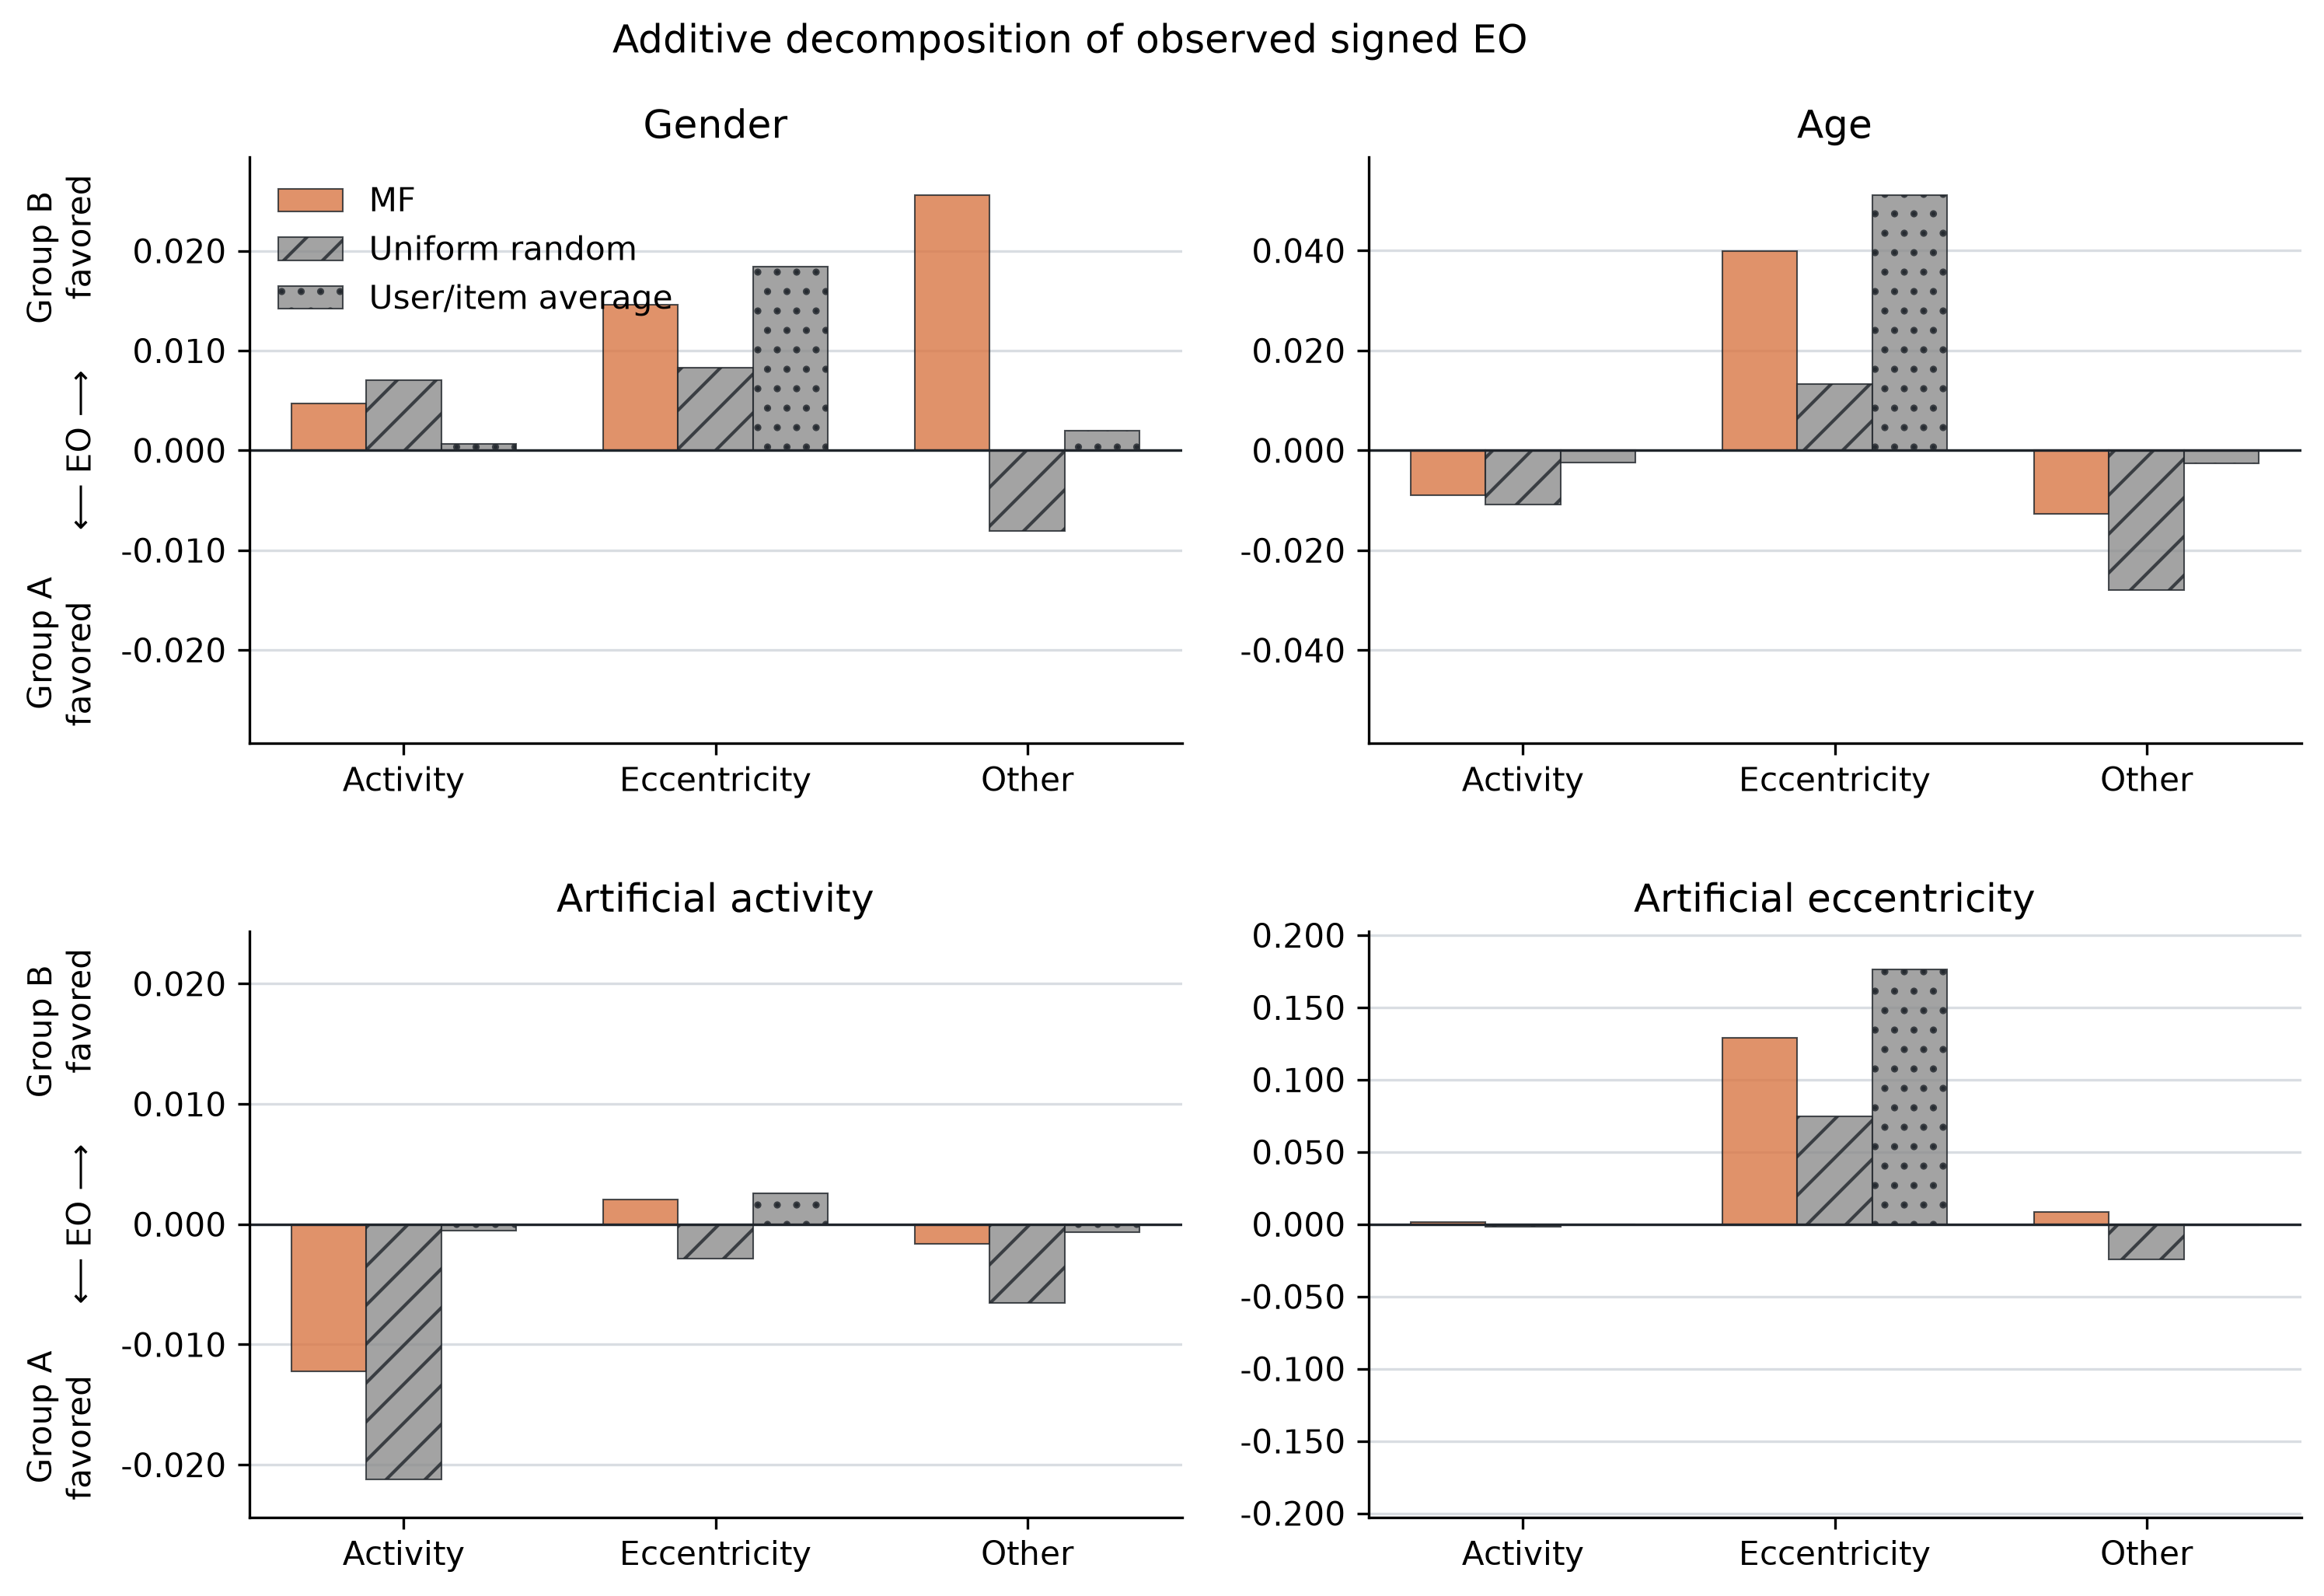
\includegraphics[width=.98\linewidth]{figures/mf_test_decomposition.png}
    \caption{Mean additive signed-EO components across the four group
    constructions and three predictors.}
    \label{fig:all-balancing-metrics}
\end{figure}

\subsection{Training-distribution intervention}

The train-side analysis examines how changing the interaction population
affects the learned model. It compares the fully balanced condition
$\mathcal T_b$ with the matched-size resized control $\mathcal T_r$ under the
common test distribution defined by the test-side weighting procedure.

\begin{table}[h]
    \centering
    \caption{Training-distribution intervention. Values are means across folds.}
    \label{tab:training-results}
    \begin{tabular}{lrrr}
        \toprule
        Condition & EO & RMSE A & RMSE B \\
        \midrule
        $\mathcal T_b$ (Fully balanced) & $0.023$ & $0.871$ & $0.894$ \\
        $\mathcal T_r$ (Resized control) & $0.042$ & $0.850$ & $0.892$ \\
        \bottomrule
    \end{tabular}
\end{table}

The balanced training population produces EO $0.023$, compared with $0.042$
for the resized control. Its RMSE for group A is $0.871$ versus $0.850$, while
group B remains similar at $0.894$ versus $0.892$. The result links training
population composition to the learned model's group error profile and shows
that this effect persists when the two training conditions have the same
rating count.

\section{Conclusion}
\label{sec:conclusion}

Global group fairness metrics alone are insufficient to interpret group error in collaborative
filtering: unequal interaction distributions can produce, reinforce, or
conceal a disparity. We proposed a distribution-aware decomposition that
addresses this gap with counterfactual alignment of rating behaviour distributions on the evaluation side and isolation of
training-population effects on the learning side, without using group
membership as a predictor feature.

Our empirical evidence, employing our group unfairness decomposition mechanism, indicates that the same apparent gap can have different
internal profiles. In the different demographic constructions in movie prediction tasks, our method was able to discern
which of the overall observed bias was caused, concealed or offset by eccentricity, activity or other psychosiciological factors being disparate between groups. Balancing population composition likewise altered the group error gap at
matched size, with unequal consequences for the two groups. 

Our findings suggest that researchers and practitioners should report group unfairness as a sum of different distributional factor contributions and residual structure
alongside aggregate bias, rather than treating the overall bias as evidence of a single unfairness
mechanism.


Further work should examine
additional rating prediction tasks and extend the analysis to multisided fairness. The scope of the evidence is limited to movie recommendation due to the unavailability of other public datasets.

\appendix
\section{Group-wise RMSE decomposition}
\label{sec:group-rmse-appendix}

The EO decomposition in Section~\ref{sec:eo-decomposition} can also be
applied separately to the RMSE of each group. The table below reports the
unweighted starting RMSE and the additive activity, eccentricity, and remaining
RMSE contributions for each construction, predictor, and group. The remaining
RMSE term represents the portion not explained by the measured activity or
eccentricity factors. The three contributions sum to the starting RMSE; a
positive contribution increases the reconstructed starting error, whereas a
negative contribution offsets it. Positive contributions are prefixed with a
plus sign in the table.

\begin{table}[H]
    \centering
    \caption{Group-wise RMSE decomposition across ten folds. The starting RMSE is decomposed into activity, eccentricity, and remaining RMSE contributions using the same Shapley construction as the EO decomposition. Positive contributions indicate increases in RMSE; negative contributions indicate decreases. Values are means $\pm$ standard deviations.}
    \label{tab:group-rmse-decomposition}
    \resizebox{\linewidth}{!}{%
    \begin{tabular}{@{}lllrrrr@{}}
        \toprule
        Construction & Predictor & Group & Starting RMSE & Activity & Eccentricity & Remaining RMSE \\
        \midrule
        \multirow{6}{*}{Gender} & MF & A & 0.833 $\pm$ 0.002 & -0.003 $\pm$ 0.002 & -0.004 $\pm$ 0.002 & 0.840 $\pm$ 0.003 \\
         &  & B & 0.878 $\pm$ 0.005 & +0.001 $\pm$ 0.002 & +0.011 $\pm$ 0.003 & 0.865 $\pm$ 0.004 \\
         & random uniform & A & 1.706 $\pm$ 0.004 & -0.005 $\pm$ 0.001 & -0.002 $\pm$ 0.002 & 1.713 $\pm$ 0.005 \\
         &  & B & 1.714 $\pm$ 0.007 & +0.002 $\pm$ 0.002 & +0.006 $\pm$ 0.002 & 1.705 $\pm$ 0.008 \\
         & user/item average & A & 0.951 $\pm$ 0.002 & -0.000 $\pm$ 0.002 & -0.004 $\pm$ 0.002 & 0.956 $\pm$ 0.004 \\
         &  & B & 0.972 $\pm$ 0.006 & +0.001 $\pm$ 0.002 & +0.014 $\pm$ 0.004 & 0.958 $\pm$ 0.004 \\
        \cline{1-3}
        \multirow{6}{*}{Age} & MF & A & 0.828 $\pm$ 0.007 & +0.003 $\pm$ 0.002 & -0.019 $\pm$ 0.002 & 0.844 $\pm$ 0.006 \\
         &  & B & 0.846 $\pm$ 0.002 & -0.006 $\pm$ 0.001 & +0.021 $\pm$ 0.002 & 0.831 $\pm$ 0.003 \\
         & random uniform & A & 1.731 $\pm$ 0.007 & +0.000 $\pm$ 0.002 & -0.002 $\pm$ 0.002 & 1.733 $\pm$ 0.007 \\
         &  & B & 1.705 $\pm$ 0.004 & -0.010 $\pm$ 0.001 & +0.011 $\pm$ 0.002 & 1.705 $\pm$ 0.005 \\
         & user/item average & A & 0.916 $\pm$ 0.005 & +0.002 $\pm$ 0.001 & -0.021 $\pm$ 0.002 & 0.934 $\pm$ 0.004 \\
         &  & B & 0.962 $\pm$ 0.002 & -0.000 $\pm$ 0.001 & +0.030 $\pm$ 0.003 & 0.932 $\pm$ 0.004 \\
        \cline{1-3}
        \multirow{6}{*}{Artificial~activity} & MF & A & 0.850 $\pm$ 0.004 & +0.006 $\pm$ 0.001 & -0.002 $\pm$ 0.003 & 0.846 $\pm$ 0.004 \\
         &  & B & 0.838 $\pm$ 0.003 & -0.007 $\pm$ 0.002 & +0.001 $\pm$ 0.002 & 0.844 $\pm$ 0.003 \\
         & random uniform & A & 1.723 $\pm$ 0.004 & +0.007 $\pm$ 0.002 & +0.001 $\pm$ 0.001 & 1.715 $\pm$ 0.005 \\
         &  & B & 1.693 $\pm$ 0.006 & -0.014 $\pm$ 0.001 & -0.002 $\pm$ 0.001 & 1.708 $\pm$ 0.006 \\
         & user/item average & A & 0.956 $\pm$ 0.004 & +0.000 $\pm$ 0.002 & -0.001 $\pm$ 0.003 & 0.957 $\pm$ 0.004 \\
         &  & B & 0.957 $\pm$ 0.003 & -0.000 $\pm$ 0.003 & +0.001 $\pm$ 0.003 & 0.956 $\pm$ 0.004 \\
        \cline{1-3}
        \multirow{6}{*}{Artificial~eccentricity} & MF & A & 0.772 $\pm$ 0.004 & -0.007 $\pm$ 0.001 & -0.036 $\pm$ 0.001 & 0.814 $\pm$ 0.004 \\
         &  & B & 0.910 $\pm$ 0.002 & -0.005 $\pm$ 0.001 & +0.093 $\pm$ 0.003 & 0.822 $\pm$ 0.003 \\
         & random uniform & A & 1.683 $\pm$ 0.004 & -0.003 $\pm$ 0.001 & -0.019 $\pm$ 0.001 & 1.705 $\pm$ 0.005 \\
         &  & B & 1.732 $\pm$ 0.006 & -0.005 $\pm$ 0.001 & +0.056 $\pm$ 0.001 & 1.681 $\pm$ 0.006 \\
         & user/item average & A & 0.864 $\pm$ 0.003 & -0.007 $\pm$ 0.001 & -0.048 $\pm$ 0.001 & 0.919 $\pm$ 0.003 \\
         &  & B & 1.040 $\pm$ 0.003 & -0.007 $\pm$ 0.001 & +0.129 $\pm$ 0.003 & 0.919 $\pm$ 0.003 \\
        \bottomrule
    \end{tabular}%
    }
\end{table}


\bibliographystyle{plain}
\bibliography{references}

\end{document}
